\documentclass[aspectratio=169,handout]{beamer}
% \usepackage[utf8]{inputenc}
\usetheme{metropolis}
\usecolortheme{orchid}
\usepackage{amsmath}
\usepackage{amssymb}
\usepackage{amsthm}
\usepackage{multirow}
\usepackage[ruled]{algorithm2e}
\usepackage{mathtools}
\usepackage{caption}
% \usepackage{epstopdf}
\usepackage{hyperref}
\setbeamerfont{footnote}{size=\tiny}

\usepackage{tikz}
\usetikzlibrary{mindmap,shadows,tikzmark,positioning,arrows.meta}

% Information boxes
\newcommand*{\info}[4][16.3]{%
  \node [ annotation, #3, scale=0.65, text width = #1em,
          inner sep = 2mm ] at (#2) {%
  \list{$\bullet$}{\topsep=0pt\itemsep=0pt\parsep=0pt
    \parskip=0pt\labelwidth=8pt\leftmargin=8pt
    \itemindent=0pt\labelsep=2pt}%
    #4
  \endlist
  };
}

\tikzset{%
  >={Latex[width=2mm,length=2mm]},
  % Specifications for style of nodes:
            base/.style = {rectangle, rounded corners, draw=black,
                           minimum width=4cm, minimum height=1cm,
                           text centered, font=\sffamily},
  activityStarts/.style = {base, fill=blue!30},
       startstop/.style = {base, fill=red!30},
    activityRuns/.style = {base, fill=green!30},
         process/.style = {base, minimum width=2.5cm, fill=orange!15,
                           font=\ttfamily},
}
\renewcommand\textbullet{\ensuremath{\bullet}}
\newcommand\scalemath[2]{\scalebox{#1}{\mbox{\ensuremath{\displaystyle #2}}}}
\newcommand{\norm}[1]{\left\lVert#1\right\rVert}

%%% Bibliography
\usepackage[citestyle=numeric,style=numeric,backend=biber,doi=false,isbn=false,url=false]{biblatex}
\addbibresource{references.bib}

%%% Suppress biblatex annoying warning
\usepackage{silence}
\WarningFilter{biblatex}{Patching footnotes failed}

%%% new theorems %%%%%%%%%%%%%%%%%%%%%%%%%%%%%%%%%%%%%%%%%%%%%%%%%%%%%%%%%%%%%%
\theoremstyle{definition}
\newtheorem{mydef}{Definition}

\theoremstyle{plain}
\newtheorem{mylemma}{Lemma}[section]
\newtheorem{mytheorem}{Theorem}[section]
\newtheorem{myproposition}{Proposition}[section]
\newtheorem{myproblem}{Problem}[section]
\newtheorem{mydefinition}{Definition}[section]
\newtheorem{myassumption}{Assumption}[section]

\theoremstyle{remark}
\newtheorem{myremark}{Remark}[section]

\newcounter{saveenumi}
\newcommand{\seti}{\setcounter{saveenumi}{\value{enumi}}}
\newcommand{\conti}{\setcounter{enumi}{\value{saveenumi}}}

\resetcounteronoverlays{saveenumi}

\title{Controles}
\subtitle{\small Clase 5: Sintonización de Controladores}
\author{Gerardo Becerra, Ph.D.}
\institute{Pontificia Universidad Javeriana\\ Departamento de Electrónica}
\date{Febrero 26, 2020}

\begin{document}

\frame{\titlepage}	

% \frame{\tableofcontents}

% \section{Tipos de Control}
\begin{frame}[<+->]\frametitle{Introducción}
\vspace*{5mm}
\centering
\begin{itemize}
	\item \textbf{Sintonización:} Selección de valores numéricos para los parámetros del controlador, con base en algún criterio.
	\item Existen muchos criterios para sintonización de controladores.
	\begin{itemize}
		\item \textcolor{green}{Experimentales}
		\item \textcolor{blue}{Análisis de la función de transferencia}
		\item \textcolor{blue}{Técnicas de optimización}
		\item \textcolor{red}{Lugar geométrico de las raíces}
		\item \textcolor{red}{Compensación en frecuencia}
	\end{itemize}
\end{itemize}
\end{frame}

\section{Análisis de la Función de Transferencia}
\begin{frame}[<+->]\frametitle{Método Matemático de Sintonización de Controladores}
\begin{enumerate}
	\item A partir de los requerimientos de desempeño, se determina un polinomio característico deseado.
	\item Se calcula la función de transferencia del sistema en lazo cerrado, en términos de los parámetros del controlador.
	\item Se comparan el polinomio característico deseado con el denominador de la función de transferencia. Si hay correspondencia en los coeficientes, se resuelve el sistema de ecuaciones para calcular los valores de los parámetros del controlador. Si no, se prueba con un controlador con una estructura diferente.
	\item Se verifica que el sistema en lazo cerrado cumpla con los requerimientos de desempeño.
\end{enumerate}
\end{frame}

\begin{frame}[c]\frametitle{Ejemplo}
Considere el modelo de segundo orden de un sistema de control de altitud de una aeronave descrito por la función de transferencia:
\begin{equation*}
	G(s) = \frac{4500}{s(s+361.2)}
\end{equation*}
Se establecen las especificaciones de desempeño como sigue:
\begin{itemize}
	\item Error en estado estable debido a una rampa $e_{ss} \leq 0.000433$.
	\item Sobrepico máximo $PO \leq 5\%$
	\item Tiempo de subida $t_r \leq 0.005$ s.
	\item Tiempo de establecimiento $t_s \leq 0.005$ s.
\end{itemize}
Determine una estructura de control PID adecuada y calcule los valores de los parámetros.
\end{frame}

\begin{frame}[<+->]\frametitle{Ejemplo}
\begin{enumerate}
	\item Polinomio característico deseado a partir de los requerimientos de desempeño.
	\begin{equation*}
		PO = 0.05 = e^{-\zeta \pi / \sqrt{1-\zeta^2}}
	\end{equation*}
	\begin{equation*}
		\zeta = 0.6901
	\end{equation*}
	Entonces, para $PO \leq 5\%$, $\zeta \geq 0.6901$. Ahora, con $t_s \leq 0.005$:
	\begin{equation*}
		\frac{4}{\zeta \omega_n} \leq 0.005 \hspace*{3mm} \Rightarrow \hspace*{3mm} \omega_n \geq \frac{4}{0.005\zeta}
	\end{equation*}
	Para $\zeta = 0.6901$, $\omega_n = 1159.2$. Entonces el polinomio característico deseado es:
	\begin{equation*}
		q(s) = s^2 + 2 \zeta \omega_n s + \omega_n^2 = s^2 + 2(0.6901)(1159.2)s + 1159.2^2 = s^2 + 1600s +1.3737\times 10^6
	\end{equation*}
	\seti
\end{enumerate}
\end{frame}

\begin{frame}[<+->]\frametitle{Ejemplo}
\begin{enumerate}
	\conti
	\item Función de transferencia en lazo cerrado en términos de los parámetros del controlador.\\
	Qué estructura debe tener el controlador? Usando controlador P:
	\begin{equation*}
		\frac{Y(s)}{R(s)} = \frac{K_p\frac{4500}{s(s+361.2)}}{1 + K_p\frac{4500}{s(s+361.2)}} = \frac{4500 K_p}{s^2 + 361.2s + 4500K_p}
	\end{equation*}
	Comparando el denominador con el polinomio característico deseado: 
	\begin{equation*}
		q(s) = s^2 + 1600s +1.3737\times 10^6
	\end{equation*}
	No hay correspondencia en el coeficiente de $s$! Entonces, no funciona utilizar el controlador P. Se debe probar con un controlador diferente.
	\seti
\end{enumerate}	
\end{frame}

\begin{frame}[<+->]\frametitle{Ejemplo}
	Usando un controlador PD:
	\begin{equation*}
		\frac{Y(s)}{R(s)} = \frac{(K_p + Kds)\frac{4500}{s(s+361.2)}}{1 + (K_p + Kds)\frac{4500}{s(s+361.2)}} = \frac{4500 (K_p + Kds)}{s^2 + (361.2+4500Kd)s + 4500K_p}
	\end{equation*}
	Al agregar el controlador D, se tiene un nuevo grado de libertad para ajustar el coeficiente de $s$. Comparando con el polinomio característico deseado:
	\begin{equation*}
		q(s) = s^2 + 1600s + 1.3737\times 10^6
	\end{equation*}
	Ahora si se puede resover el sistema de ecuaciones.
\end{frame}

\begin{frame}[<+->]\frametitle{Ejemplo}
\begin{enumerate}
	\conti
	\item Comparando los coeficientes de los dos polinomios:
	\begin{align*}
		&s^2 + (361.2+4500Kd)s + 4500K_p\\
		&s^2 + 1600s +1.3737\times 10^6
	\end{align*}
	Se tiene el sistema de ecuaciones
	\begin{align*}
		4500K_p = 1.3737\times 10^6\\
		361.2+4500Kd = 1600
	\end{align*}
	Entonces:
	\begin{align*}
		K_p = 298.6099\\
		K_d = 0.2753
	\end{align*}
	\seti
\end{enumerate}
\end{frame}

\begin{frame}[<+->]\frametitle{Ejemplo}
	\begin{enumerate}
		\conti
		\item Verificar que se cumplan los requerimientos de desempeño.\\
		\vspace*{5mm}
		Se puede usar una simulación para verificarlo...
	\end{enumerate}
\end{frame}

\begin{frame}[c]\frametitle{Ejercicio 1}
Considere el sistema descrito por
\begin{equation*}
	G(s) = \frac{2}{s^2 + 0.03s + 2.25}
\end{equation*}
Diseñe un controlador tal que el sistema tenga
\begin{enumerate}
	\item Error en estado estable nulo ante escalón unitario.
	\item Sobrepico $\leq 10\%$ .
	\item Tiempo de establecimiento $t_s \leq 10$ s.
\end{enumerate}
\end{frame}

\section{Técnicas de Optimización}
\begin{frame}[<+->]\frametitle{Índices de Desempeño}
	\begin{columns}
	\begin{column}{0.5\textwidth}
	\begin{itemize}
		\item Integral del cuadrado del error (ISE):
		\begin{equation*}
			ISE = \int_0^T e^2(t) dt
		\end{equation*}
		\item Integral del valor absoluto del error (IAE):
		\begin{equation*}
			IAE = \int_0^T |e(t)| dt
		\end{equation*}
	\end{itemize}
	\end{column}	
	\begin{column}{0.5\textwidth}
	\begin{itemize}
		\item Integral del valor absoluto del error ponderado en el tiempo (ITAE):
		\begin{equation*}
			ITAE = \int_0^T t |e(t)| dt
		\end{equation*}
		\item Integral del cuadrado del error ponderado en el tiempo (ITSE):
		\begin{equation*}
			ITAE = \int_0^T t e^2(t) dt
		\end{equation*}
	\end{itemize}
	\end{column}	
	\end{columns}
	\vspace*{-5mm}
	\textbf{Objetivo:} seleccionar parámetros del sistema para minimizar algún índice de desempeño.
	% $T$: Es conveniente seleccionarlo como el tiempo de establecimiento $T_s$.
\end{frame}
\begin{frame}[<+->]\frametitle{Minimización de los Índices de Desempeño}
\begin{itemize}
	\item Sistema de control $\rightarrow$ es óptimo cuando se minimiza algún índice de desempeño seleccionado.
	\item Valor óptimo de los parámetros $\rightarrow$ depende del índice de desempeño.
	\item Para la función de transferencia de lazo cerrado de la forma general:
	\begin{equation*}
		T(s) = \frac{Y(s)}{R(s)} = \frac{b_0}{s^n + b_{n-1} s^{n-1} + \dots + b_1 s + b_0}
	\end{equation*}
	se han determinado los coeficientes óptimos que minimizan el ITAE para una entrada paso.
	\item Ésta función de transferencia tiene $e_{ss} = 0$ para entrada paso.
\end{itemize}
\end{frame}

\begin{frame}[<+->]\frametitle{Coeficientes Óptimos Basados en el Criterio ITAE para una Entrada Paso}
\centering
\begin{equation*}
	T(s) = \frac{Y(s)}{R(s)} = \frac{b_0}{s^n + b_{n-1} s^{n-1} + \dots + b_1 s + b_0}
\end{equation*}
\vspace*{10mm}

\includegraphics[width=10cm]{images/optimCoeffsITAEstep.eps}
\end{frame}

\begin{frame}[<+->]\frametitle{Coeficientes Óptimos Basados en el Criterio ITAE para una Entrada Rampa}
\centering
\begin{equation*}
	T(s) = \frac{Y(s)}{R(s)} = \frac{b_1s + b_0}{s^n + b_{n-1} s^{n-1} + \dots + b_1 s + b_0}
\end{equation*}
\vspace*{10mm}

\includegraphics[width=8cm]{images/optimCoeffsITAEramp.eps} 
\end{frame}

\begin{frame}[c]\frametitle{Respuesta Paso para Coeficientes Óptimos Basados en Criterio IAE}
\vspace*{5mm}
\centering
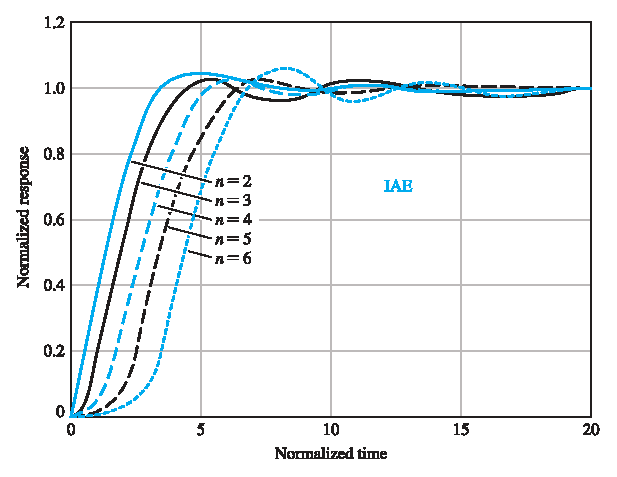
\includegraphics[width=8cm]{images/stepResponseOptimIAE.eps}
\end{frame}

\begin{frame}[c]\frametitle{Respuesta Paso para Coeficientes Óptimos Basados en Criterio ITAE}
\vspace*{5mm}
\centering
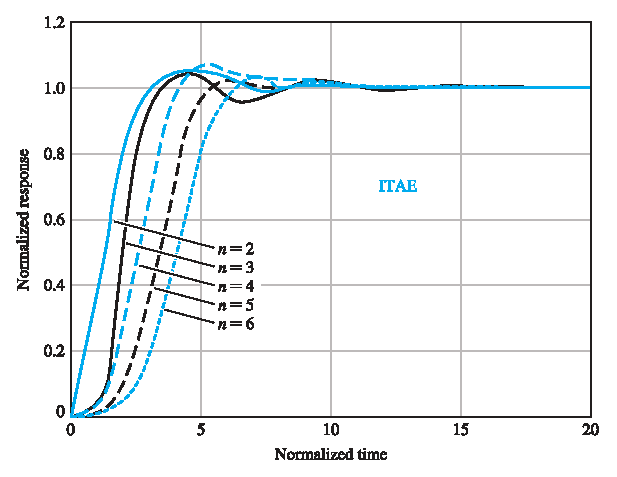
\includegraphics[width=8cm]{images/stepResponseOptimITAE.eps}
\end{frame}

\begin{frame}[c]\frametitle{Respuesta Paso para Coeficientes Óptimos Basados en Criterio ISE}
\vspace*{5mm}
\centering
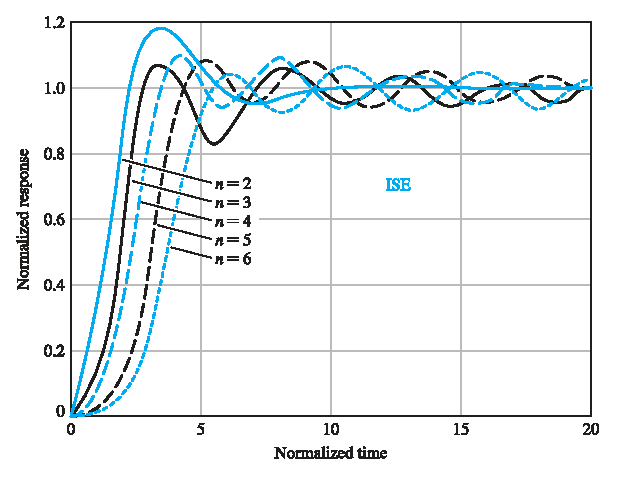
\includegraphics[width=8cm]{images/stepResponseOptimISE.eps}
\end{frame}

\begin{frame}[<+->]\frametitle{Diseño de Controladores usando Coeficientes Óptimos - Ejemplo}
Considere el sistema
\begin{equation*}
	G(s) = \frac{1}{s(s+2)}
\end{equation*}
Encuentre un sistema de cero error de posición que minimice el criterio ITAE. También se requiere que la señal de control debida a una señal escalón unitario satisfaga $|u(t)| \leq 3$.\\
\vspace*{3mm}
La función de transferencia óptima a partir de la tabla se selecciona como:
\begin{equation*}
	\frac{Y(s)}{R(s)} = G_0 = \frac{\omega_n^2}{s^2 + 1.4 \omega_n s + \omega_n^2}
\end{equation*}
Note que aumentando $\omega_n$, aumentan la velocidad de respuesta y la señal de control. Se debe seleccionar $\omega_n$ tal que $|u(t)| \leq 3$.
\end{frame}

\begin{frame}[<+->]\frametitle{Diseño de Controladores usando Coeficientes Óptimos - Ejemplo}
La función de transferencia desde $R(s)$ hasta $U(s)$ es
\begin{equation*}
	\frac{U(s)}{R(s)} = \frac{G_0(s)}{G(s)} = \frac{\omega_n^2 s (s+2)}{s^2 + 1.4 \omega_n s + \omega_n^2}
\end{equation*}
\begin{equation*}
	U(s) = \frac{\omega_n^2 s (s+2)}{s^2 + 1.4 \omega_n s + \omega_n^2} R(s)
\end{equation*}
Usando simulación, se encuentra que el máximo valor de $u(t)$ ocurre en $t = 0^+$. Para encontrar dicho valor se usa el teorema del valor inicial:
\begin{equation*}
	u_{max} = u(0^+) = \lim_{s \rightarrow \infty} s U(s) = \lim_{s \rightarrow \infty} s \frac{\omega_n^2 s (s+2)}{s^2 + 1.4 \omega_n s + \omega_n^2} \frac{1}{s} = \omega_n^2
\end{equation*}
Entonces, para satisfacer $|u(t)| \leq 3$ se requiere $\omega_n^2 = 3$. Entonces el sistema ITAE óptimo es:
\begin{equation*}
	\frac{Y(s)}{R(s)} = \frac{3}{s^2 + 1.4 \sqrt{3} s + 3} = \frac{3}{s^2 + 2.4 s + 3} 
\end{equation*}
\end{frame}

\begin{frame}[c]\frametitle{Ejercicio 2}
Considere una planta con función de transferencia $2/s^2$. Encuentre un sistema óptimo que minimice el criterio ITAE bajo la restricción $|u(t)| \leq 3$.
\end{frame}

\begin{frame}[c]\frametitle{Ejercicio 3}
Considere una planta con función de transferencia $2/s^2$. Encuentre un sistema óptimo que minimice el criterio ITAE bajo la restricción $|u(t)| \leq 3$ y que el error de velocidad sea cero.
\end{frame}

\begin{frame}[c]\frametitle{Ejercicio 4}
Considere una planta cuya función de transferencia es
\begin{equation*}
	G(s) = \frac{2}{s(s^2 + 0.25s + 6.25)}
\end{equation*}
Encuentre un sistema óptimo ITAE de error de posición cero. Se requiere que la señal de control $u(t)$ debida a una señal de entrada escalón unitario satisfaga $|u(t)| \leq 10$.
\end{frame}

\end{document}